\documentclass[conference]{IEEEtran}

\usepackage{amsmath}
\usepackage{amssymb}
\usepackage{booktabs}
\usepackage{array}
\usepackage{graphicx}
\usepackage{multirow}
\usepackage{url}
\usepackage{cite}
\usepackage{xcolor}
\usepackage{xspace}
\usepackage[hidelinks]{hyperref}
\usepackage{tikz}
\usetikzlibrary{positioning,arrows.meta,fit,calc,backgrounds}
\usepackage{tabularx}
\usepackage{threeparttable}

\newcommand{\code}[1]{\texttt{#1}}

\def\BibTeX{{\rm B\kern-.05em{\sc i\kern-.025em b}\kern-.08em
    T\kern-.1667em\lower.7ex\hbox{E}\kern-.125emX}}

% Global Float Padding Reduction
\setlength{\textfloatsep}{6pt plus 1.0pt minus 2.0pt}
\setlength{\floatsep}{6pt plus 1.0pt minus 2.0pt}
\setlength{\intextsep}{6pt plus 1.0pt minus 2.0pt}


\begin{document}

\title{AuthGuard-7702: Robust Pre-Authorization Screening of EIP-7702 Delegate Bytecode}



\maketitle

\begin{abstract}
Ethereum's EIP-7702 creates a security decision point before a user authorizes smart-contract code to execute through an externally owned account. At that point, behavioral history, reputation, or verified source code may be unavailable, while deployed runtime bytecode is observable. We present AuthGuard-7702, a bytecode-only pre-authorization screening framework, and AuthGuard-Seq, a 30,050-parameter hierarchical opcode model with shared local convolutions and learned chunk attention. Evaluation uses 2,190 observed delegates in 790 bytecode-similarity families, five family-disjoint folds, and three seeds. A parameter-matched study separates input budget, hierarchy, and aggregation. On clean bytecode, a 16K flat control obtains 0.936 AUPRC and AuthGuard-Seq obtains 0.918; learned attention nevertheless improves over mean aggregation by 0.039 AUPRC with a fold-stratified family-bootstrap 95\% interval of [0.007, 0.064]. Under cap-correct 200\% donor flooding, AuthGuard-Seq retains 0.908 AUPRC and exceeds the matched 16K flat control by 0.098 [0.059, 0.154]. Its nominal-5\%-FPR threshold transfers to 797 external benign controls with $0.059\pm0.007$ observed FPR. A saved checkpoint occupies 125,300 bytes, and the complete measured local CPU path has 2.942 ms median latency. These results support learned chunk aggregation as a compact robustness mechanism while showing that hierarchy is not universally superior on clean inputs.
\end{abstract}

\begin{IEEEkeywords}
EIP-7702, Ethereum, smart contract security, bytecode analysis, machine learning
\end{IEEEkeywords}

\section{Introduction}
\label{sec:intro}

Ethereum traditionally distinguishes externally owned accounts (EOAs), which are controlled by users, from smart contracts that contain executable logic. EIP-7702 modifies this model by allowing an EOA to delegate code execution while retaining its original address~\cite{eip7702}. This enables account-abstraction capabilities such as transaction batching, gas sponsorship, and programmable authorization, but it also creates a new trust boundary. Authorizing unsafe delegate code can allow untrusted smart-contract logic to access or manipulate the EOA's state, assets, approvals, and transaction behavior.

The critical decision occurs before authorization. A newly proposed delegate may have little transaction history, no established reputation, and no verified source code, yet its deployed runtime bytecode can already be retrieved from the blockchain. Existing EIP-7702 studies document delegation-based phishing, persistent compromise, and related risks~\cite{qi2025eip7702,huang2026darkside}, but primarily emphasize ecosystem-scale detection, transaction evidence, static program analysis, or protocol defenses. In parallel, machine-learning studies show that EVM bytecode and opcode representations contain useful signals for vulnerability and phishing detection~\cite{phishinghook2025,contractward2021,eth2vec2022}. These approaches do not address the distinct operational decision of whether a proposed EIP-7702 delegate should be authorized. Figure~\ref{fig:riskwindow} illustrates this authorization risk window. The wallet can retrieve delegate runtime bytecode before signature, while behavioral, reputation-based, or source-level evidence may still be unavailable.

\begin{figure}[t]
\centering
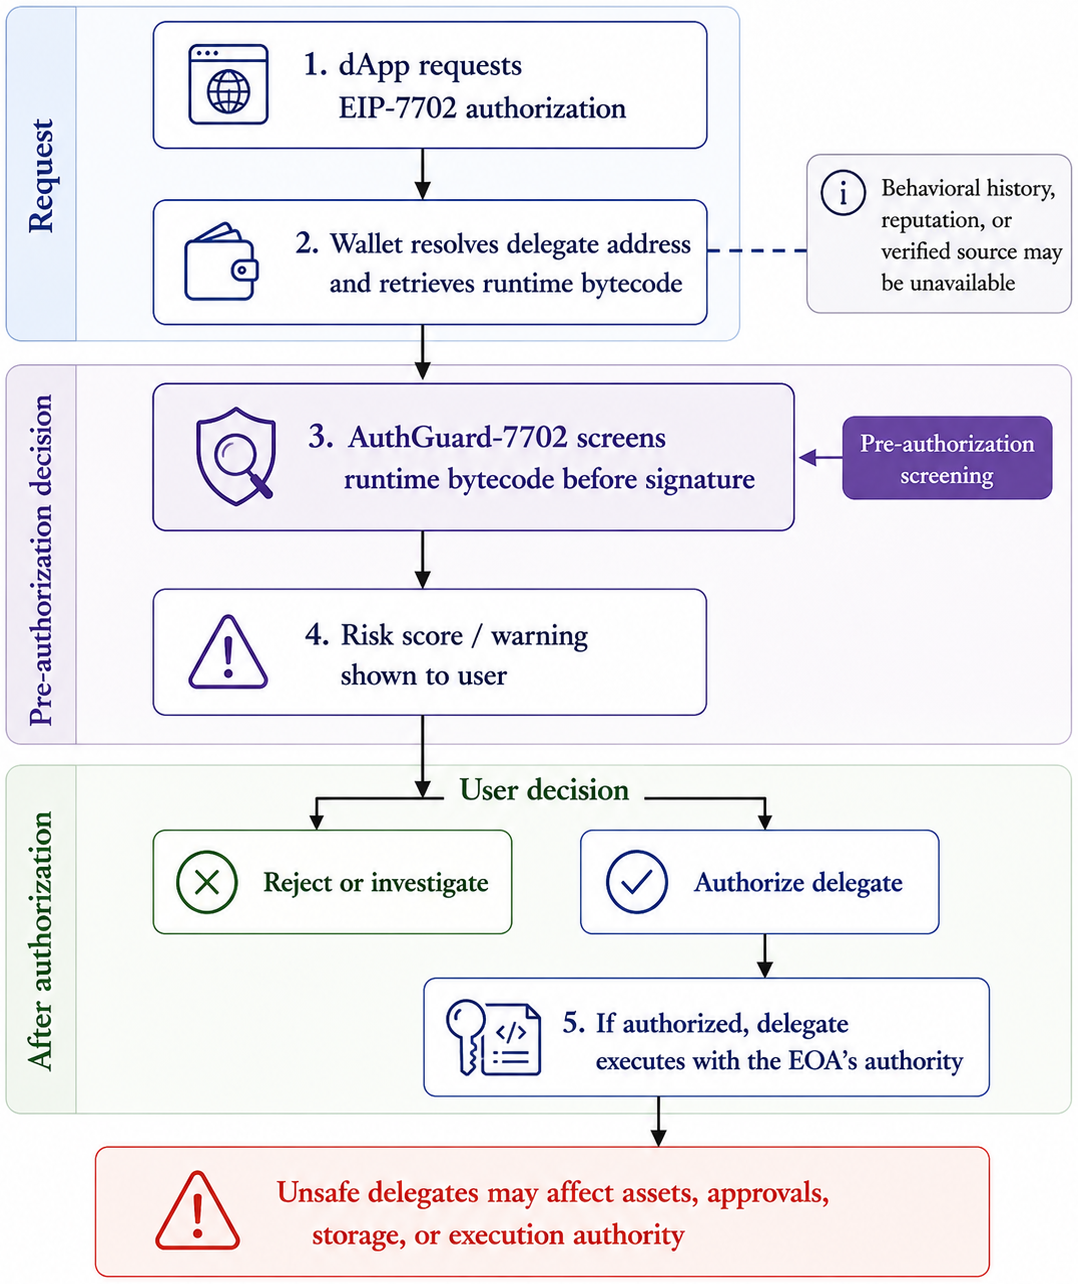
\includegraphics[width=\columnwidth]{eip_7702_authorization_risk_flowchart.png}
\caption{EIP-7702 authorization flow}
\label{fig:riskwindow}
\end{figure}

We address this gap with AuthGuard-7702, a bytecode-only pre-authorization screening framework that produces a calibrated screening score and warning tier. Its central model, AuthGuard-Seq, disassembles runtime bytecode, partitions the opcode stream into 256-token chunks, encodes local ordered patterns using shared convolutions, and learns attention weights that aggregate evidence across chunks. The model processes up to 16,384 opcodes, which is sufficient for every program in the audited benchmark, without using transaction history, source code, address identity, or reputation metadata. This additional context is material in the study population: 712 of 2,190 delegates (32.5\%) exceed the 2,048-opcode view used by the Flat CNN and BiGRU baselines.

A second methodological challenge is dependence among smart-contract samples. Code duplication can inflate the measured performance of machine-learning models of code~\cite{allamanis2019duplication}. Smart-contract datasets may likewise contain identical redeployments and closely related bytecode variants, allowing row-level random splits to place near-duplicate programs in both training and test data and thereby overstate generalization~\cite{tesseract2019}. We therefore audit the source data, construct bytecode-similarity families, prevent identical bytecode and related families from crossing folds, and exclude observations with unreliable source verdicts. We also compare flat, mean-pooled, and attention-pooled encoders at matched parameter and token budgets. The resulting evidence does not support universal clean superiority for hierarchy: the 16K flat control is strongest on clean AUPRC. It does support learned attention over mean aggregation on clean inputs and a 0.098 AUPRC advantage over the matched flat control under cap-correct Flood-200\%. This clean--robustness tradeoff is central to the revised evaluation.

The study makes three primary contributions:
\begin{itemize}
    \item We introduce a bytecode-only machine-learning framework for screening proposed EIP-7702 delegates before authorization, without requiring transaction history, reputation, identity, or verified source code.
    \item We develop a compact 30,050-parameter hierarchical encoder and a parameter-matched study that isolates context budget, hierarchy, and learned aggregation. The study identifies attention as a supported robustness mechanism rather than claiming universal clean superiority.
    \item We construct an audited benchmark and leakage-resistant evaluation combining bytecode-family folds, validation-only operating points, donor-isolated fixed-cap flooding, fold-stratified family bootstrap intervals, external controls, and complete-path latency.
\end{itemize}

\section{Background and Related Work}
\label{sec:related}
This section reviews the EIP-7702 authorization model and positions AuthGuard-7702 relative to prior bytecode learning, static analysis, and security-ML evaluation methodology.

\subsection{EIP-7702 and the Authorization Boundary}

EIP-7702 introduces authorization tuples through which an EOA can delegate code execution while retaining its original address. For each valid tuple, a delegation indicator formatted as $\code{0xef0100}\Vert\code{address}$ is written to the authorizing EOA's code field. Subsequent code-executing operations resolve and execute the code at the referenced delegate address~\cite{eip7702}. The security-relevant object for screening is therefore the delegate's executable runtime bytecode rather than the 23-byte indicator itself. Once authorized, the referenced code can execute in the EOA's context, making the pre-signature decision a natural point for automated screening.

Huang et al. combine transaction analysis with cross-contract static analysis to characterize EIP-7702-related malicious behavior~\cite{huang2026darkside}, while Qi et al. study delegation-based phishing mechanisms and protocol-level defenses~\cite{qi2025eip7702}. To the best of our knowledge, neither work investigates machine-learning-based screening of proposed delegate bytecode before authorization.

\subsection{Learning from Smart-Contract Bytecode}

Prior learning-based methods demonstrate that EVM representations can support security classification. ContractWard uses opcode bigrams with conventional learners~\cite{contractward2021}, Eth2Vec learns contract-wide bytecode representations~\cite{eth2vec2022}, and PhishingHook evaluates bytecode and opcode representations for phishing-contract classification~\cite{phishinghook2025}. More recent work combines bytecode-derived features with control-flow-graph analysis~\cite{smartbugbert2025}, while surveys emphasize representation, dataset construction, and evaluation design as recurring determinants of reported performance~\cite{wang2026review}. PhishingHook is particularly relevant because it shows that predictive security signals can be learned directly from EVM bytecode without transaction analysis. AuthGuard-7702 addresses a different operational setting by screening a proposed EIP-7702 delegate before authorization, and its primary benchmark consists entirely of observed delegates drawn from a common acquisition pipeline. Table~\ref{tab:related} summarizes this positioning.

\begin{table}[t]
\centering
\caption{Comparison with representative prior work}
\label{tab:related}
\begin{threeparttable}
\scriptsize
\begin{tabularx}{\columnwidth}{@{}X c c c@{}}
\toprule
Work & EIP-7702 & Bytecode ML & Pre-authorization screening \\
\midrule
Huang et al.~\cite{huang2026darkside} & \checkmark & -- & -- \\
Qi et al.~\cite{qi2025eip7702} & \checkmark & -- & -- \\
PhishingHook~\cite{phishinghook2025} & -- & \checkmark & -- \\
Eth2Vec~\cite{eth2vec2022} & -- & \checkmark & -- \\
\textbf{AuthGuard-7702} & \checkmark & \checkmark & \checkmark \\
\bottomrule
\end{tabularx}
\begin{tablenotes}[flushleft]
\scriptsize
\item[] ``Bytecode ML'' denotes machine learning directly over bytecode or opcode representations. ``Pre-authorization screening'' denotes automated risk assessment of proposed delegate code before authorization.
\end{tablenotes}
\end{threeparttable}
\end{table}

\subsection{Static Analysis and Security-ML Evaluation}

Bytecode learning complements rather than replaces semantic analysis. Gigahorse decompiles EVM bytecode for declarative analysis~\cite{gigahorse2019}, while Securify derives semantic dependencies and checks security patterns~\cite{securify2018}. The reference labels originate from a decompiler-based rule~\cite{huang2026darkside}, but our question is whether that signal can be approximated directly from opcode sequences by a lightweight pre-authorization screener. Evaluation methodology is equally important. TESSERACT shows how dependence and distribution bias can inflate security-classification results~\cite{tesseract2019}. We therefore isolate identical and similar bytecode families across folds and interpret transformed executable inputs only within their demonstrated preservation guarantees, consistent with problem-space adversarial-ML guidance~\cite{pierazzi2020}.



\begin{figure*}[t]
\centering
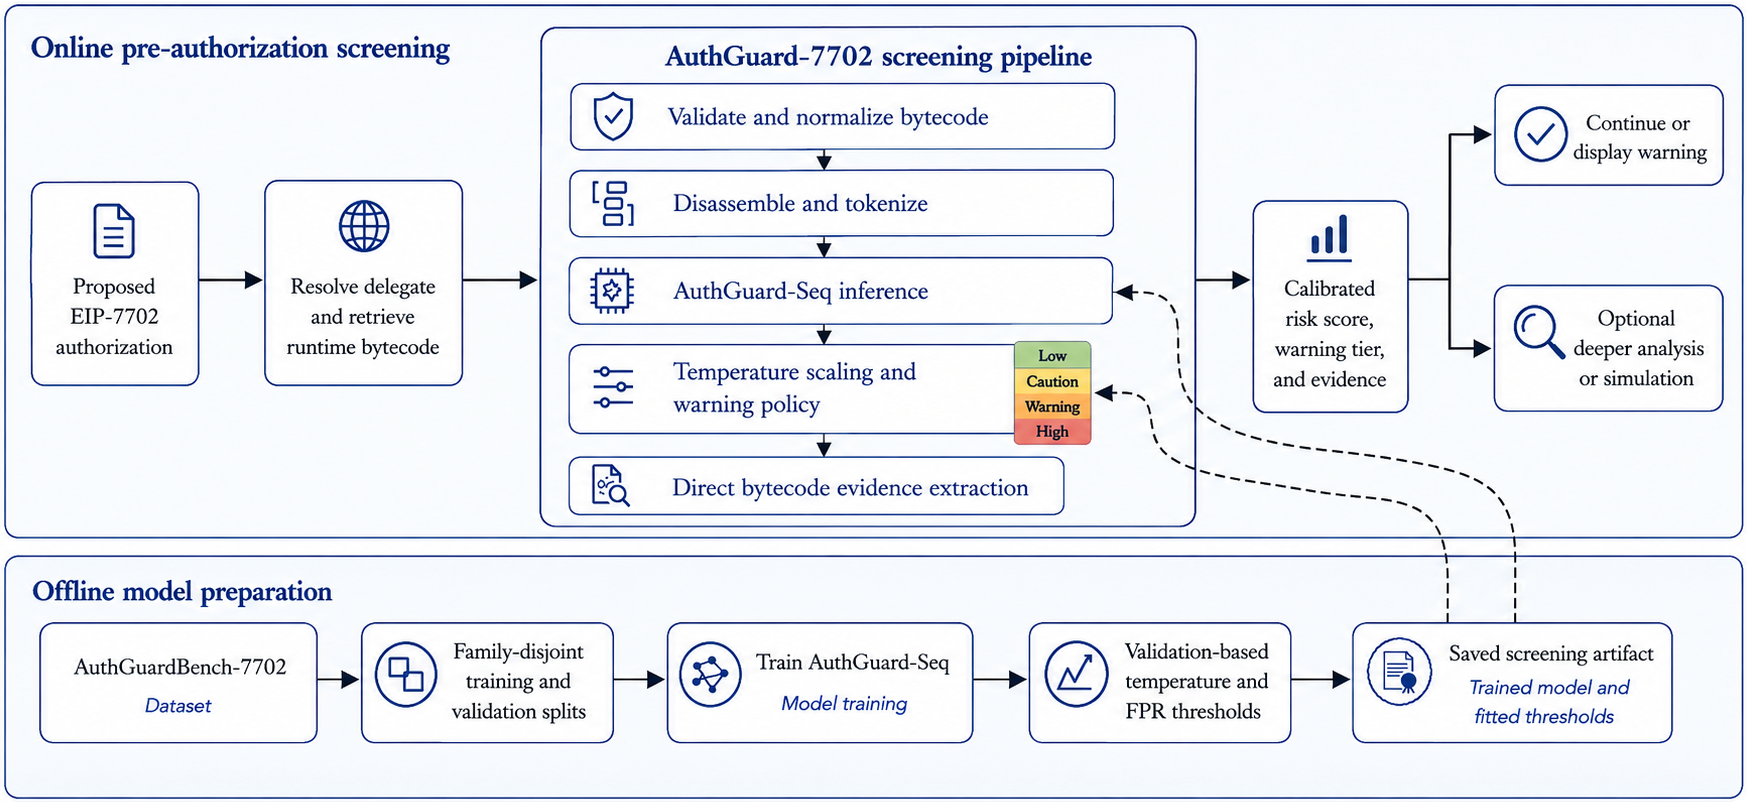
\includegraphics[width=0.98\textwidth]{figure-1-bak.png}
\caption{AuthGuard-7702 system overview}
\label{fig:decision}
\end{figure*}



\section{Problem Formulation and Threat Model}
\label{sec:problem}
This section defines the pre-authorization screening task, the model's information boundary, and the assumed attacker and defender capabilities.


\subsection{Pre-Authorization Screening Task}

Let $b$ denote the normalized runtime bytecode at a proposed delegate address and let $T(b)$ denote its opcode-token sequence. A trained model $f_\theta$ produces a risk logit that is temperature-scaled using validation data~\cite{guo2017calibration}:

\begin{equation}
s(b)=\sigma\left(\frac{f_\theta(T(b))}{T_{\mathrm{cal}}}\right),
\qquad
T_{\mathrm{cal}}>0,
\qquad
s(b)\in[0,1].
\label{eq:score}
\end{equation}

The resulting value $s(b)$ is a calibrated model score indicating the strength of evidence that the delegate contains opcode patterns associated with the benchmark's reference risk condition. The positive class consists of delegates flagged by the source study's static-analysis rule, which identifies decompiled reachability from standardized inbound hooks, including \code{receive()}, \code{fallback()}, and token-reception callbacks, to predefined value-moving external-call patterns~\cite{huang2026darkside}. The negative class consists of delegates from the same source pool that were not flagged. Because an unflagged verdict does not establish benign semantics, the task is screening for source-analyzer-identified risk rather than proving malicious intent, exploitability, or delegate safety.

From negative validation scores, we derive thresholds $\tau_1\geq\tau_5\geq\tau_{10}$ for nominal 1\%, 5\%, and 10\% FPR operating points. Scores $s\geq\tau_1$ map to \textsc{High}, $\tau_5\leq s<\tau_1$ to \textsc{Warning}, $\tau_{10}\leq s<\tau_5$ to \textsc{Caution}, and $s<\tau_{10}$ to \textsc{Low-Observed-Risk}. Because thresholds are estimated from finite validation sets, held-out FPR can differ from the nominal target.

\subsection{Information Boundary}

The core model observes only the ordered opcode sequence derived from runtime bytecode. PUSH immediate operands are skipped, so the sequence representation captures opcode identities and ordering rather than embedded constants. The model receives no transaction history, balances or approvals, graph or address identity, source code, family or fold identifiers, or fields used to construct the reference labels. This boundary is deliberate because the intended use case is a delegate that may lack historical or identity-based evidence at authorization time. The component is an advisory first-stage screener and does not resolve proxy state, simulate transactions, infer off-chain intent, or certify authorization safety. Those signals can be supplied by downstream security systems after initial triage.


\begin{figure*}[t]
\centering
\resizebox{0.98\textwidth}{!}{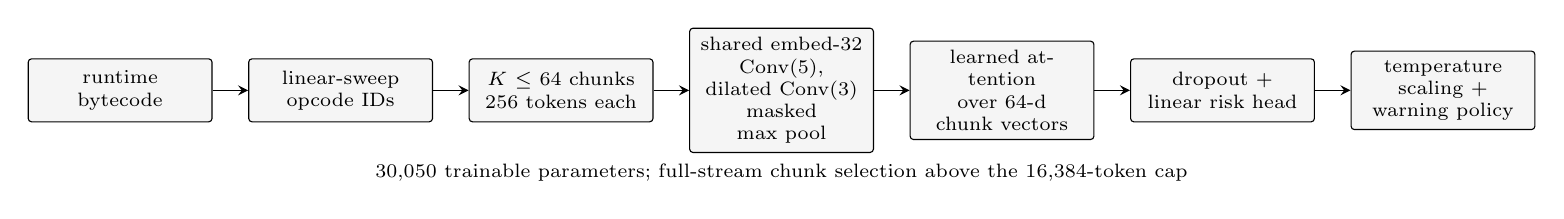
\begin{tikzpicture}[
  font=\scriptsize,
  box/.style={draw, rounded corners=1.2pt, minimum height=8mm, text width=21mm,
              align=center, fill=gray!8},
  flow/.style={->, >=stealth, line width=.6pt}
]
  \node[box] (bytecode) at (0,0) {runtime bytecode};
  \node[box] (tokens) at (2.8,0) {linear-sweep opcode IDs};
  \node[box] (chunks) at (5.6,0) {$K\leq64$ chunks\\256 tokens each};
  \node[box] (local) at (8.4,0) {shared embed-32\\Conv(5), dilated Conv(3)\\masked max pool};
  \node[box] (attn) at (11.2,0) {learned attention\\over 64-d chunk vectors};
  \node[box] (head) at (14.0,0) {dropout + linear risk head};
  \node[box] (policy) at (16.8,0) {temperature scaling + warning policy};
  \draw[flow] (bytecode) -- (tokens);
  \draw[flow] (tokens) -- (chunks);
  \draw[flow] (chunks) -- (local);
  \draw[flow] (local) -- (attn);
  \draw[flow] (attn) -- (head);
  \draw[flow] (head) -- (policy);
  \node[align=center] at (8.4,-1.05) {30,050 trainable parameters; full-stream chunk selection above the 16,384-token cap};
\end{tikzpicture}
}
\caption{Promoted AuthGuard-Seq architecture. All controlled neural variants reuse the same local encoder and risk head; only input layout, budget, and chunk aggregation change.}
\label{fig:encoder}
\end{figure*}



\subsection{Threat Model}

We consider an adversary who attempts to induce authorization of a delegate whose runtime code exhibits the reference risk condition. The adversary may control the deployed bytecode and modify layout, appended content, metadata, or other representation-level features to evade bytecode screening. The defender is a wallet or security service that retrieves the proposed delegate's on-chain runtime bytecode and applies AuthGuard-7702 before authorization. We assume correct bytecode retrieval and trusted model parameters and screening code. Compromise of the wallet, signing key, retrieval infrastructure, or screener is outside scope.

The model can detect only risk signals observable from runtime bytecode. Behavior that depends primarily on dynamic state, transaction-specific context, unresolved proxy targets, external counterparties, or off-chain intent may remain invisible. Our robustness experiments therefore test selected representation-level modifications rather than universal robustness to arbitrary semantics-preserving or adaptive white-box transformations.



\section{AuthGuard-7702}
\label{sec:system}
This section presents the AuthGuard-7702 screening workflow and the compact hierarchical AuthGuard-Seq model used to assess delegate bytecode.



\subsection{Screening Workflow}

Figure~\ref{fig:decision} places AuthGuard-7702 at the EIP-7702 authorization boundary. A wallet or security service resolves the proposed delegate address, retrieves its runtime bytecode, and invokes the local screening path before the user authorizes it. The pipeline normalizes and disassembles the bytecode, runs AuthGuard-Seq, applies validation-fitted calibration and thresholds, and returns a risk score, warning tier, and auxiliary bytecode evidence. Elevated scores can trigger a wallet warning or deeper analysis before the authorization decision. During model development and evaluation, the offline path constructs family-disjoint folds, trains AuthGuard-Seq, and fits the temperature-scaling parameter and FPR thresholds using validation data only. The trained model, calibration parameter, and thresholds are then stored as the screening artifact used by the online path.



The auxiliary evidence is extracted separately from the raw bytecode and includes directly observed properties such as code length, opcode counts, call-family instructions, storage writes, contract-creation instructions, and recognized token-transfer or approval selectors. These observations and the learned attention weights provide context about influential bytecode regions, but they should not be interpreted as causal explanations or control-flow proofs.

\subsection{Design Requirements and Screening Semantics}

AuthGuard-7702 is designed as a bounded triage layer rather than a learned replacement for semantic analysis. The benchmark label encodes a decompiler-derived structural risk condition, while the deployed model receives only runtime opcode order. The learning problem is therefore deliberately constrained to determining whether a previously unseen delegate contains bytecode patterns associated with the reference condition without access to decompiler outputs, transaction history, source code, or identity information.

Table~\ref{tab:design-map} maps the principal deployment requirements to the mechanisms used by AuthGuard-Seq. Local convolutions preserve short opcode-order motifs, chunking supports long runtime programs, learned attention combines evidence distributed across chunks, and validation-fitted calibration and thresholds convert the raw model output into an operational warning policy.



At screening time, the saved model and calibration artifact are applied to the runtime bytecode resolved from the proposed delegate. A \textsc{Low-Observed-Risk} tier means only that the calibrated score lies below the lowest validation-derived threshold.  Higher tiers indicate progressively stronger model evidence and can be used by a wallet to display a warning or escalate the delegate to simulation, static analysis, or human review before authorization. Because the thresholds are fitted to validation FPR targets, their realized false-positive rates may shift when applied to a different contract population. RQ3 evaluates this transfer using an external benign-control population.



\begin{table}[t]
\centering
\caption{AuthGuard-Seq design requirements and corresponding mechanisms}
\label{tab:design-map}
\scriptsize
\begin{tabularx}{\columnwidth}{@{}X X X@{}}
\toprule
Requirement & Mechanism & Role \\
\midrule
Pre-authorization, bytecode-only use & Deterministic disassembly and opcode tokens & Operates without history or source code \\
Preserve local instruction order & Shared and dilated 1-D convolutions & Captures short ordered opcode motifs \\
Cover long runtime programs & Up to $64\times256$ opcode chunks & Processes up to 16,384 tokens without prefix-only truncation \\
Combine distributed evidence & Learned chunk attention & Produces a contract-level representation \\
Operational warning policy & Temperature scaling and validation-derived FPR thresholds & Maps calibrated scores to warning tiers \\
\bottomrule
\end{tabularx}
\end{table}



\subsection{Hierarchical Opcode-Sequence Model}

AuthGuard-Seq implements the preceding requirements using shared local convolutional encoders and contract-level chunk attention. The local encoders capture short ordered opcode patterns, while chunking and attention aggregate evidence across the processed runtime sequence. It begins with deterministic linear-sweep EVM disassembly. Recognized opcodes map to stable token IDs, undefined byte values use a dedicated token, and padding uses a separate ID. PUSH immediate operands are skipped according to their instruction widths. Tokenization does not terminate at the first linear \code{STOP} instruction, so trailing bytecode regions are not discarded solely because of an early stopping opcode. In a separate bounded audit of ten delegates and 100 fixed calls, 92 calls executed an instruction after the first linear \code{STOP}, while first-\code{STOP} truncation preserved the recorded execution fingerprint in only 22 calls. We therefore treat first-\code{STOP} truncation as semantically unsafe rather than as executable-bytecode canonicalization. The resulting opcode sequence is divided into chunks of length $L=256$, with at most $K=64$ chunks. The longest benchmark program contains 10,795 opcode tokens (16,136 runtime bytes) and therefore fits within the model's 16,384-token capacity. Every benchmark contract is consequently processed in full. For longer contracts outside the benchmark, the model retains evenly spaced chunks rather than using prefix-only truncation.

Each chunk is embedded into 32 dimensions, processed by a kernel-5 convolution followed by a kernel-3 dilated convolution with dilation 2, and reduced through masked maximum pooling to a 64-dimensional representation $h_k$. Learned attention aggregates the valid chunk representations:

\begin{equation}
\alpha_k=\frac{\exp(w^\top h_k)}{\sum_{j=1}^{K_b}\exp(w^\top h_j)},
\qquad
h=\sum_{k=1}^{K_b}\alpha_k h_k,
\label{eq:attention}
\end{equation}


where $w$ is a learned vector and $K_b$ is the number of non-padding chunks. Larger values of $\alpha_k$ indicate greater learned relevance of chunk $k$ to the contract-level representation, but they are not causal explanations. The aggregated 64-dimensional vector passes through dropout and a linear binary risk head. AuthGuard-Seq contains 30,050 trainable parameters; the attention scorer accounts for only 65 of them. Its risk logit is temperature-scaled before the validation-derived warning thresholds are applied. Figure~\ref{fig:encoder} summarizes the promoted architecture.




\section{Benchmark and Experimental Methodology}
\label{sec:method}
This section describes benchmark construction, family-disjoint evaluation, baselines, training, robustness testing, statistical analysis, and local timing measurement.

\subsection{Audited Benchmark Construction}

AuthGuardBench-7702 contains 3,082 audited observations partitioned into four populations before evaluation. The primary population comes from the EIP-7702 delegate dataset and analyzer outputs released by Huang et al.~\cite{huang2026darkside}. After auditing and filtering, it contains 2,190 delegates, including 727 source-analyzer-flagged and 1,463 source-unflagged observations. The external control contains 797 benign-labeled general Ethereum contracts from the PhishingHook-derived source~\cite{phishinghook2025}. Five manually curated legitimate EIP-7702 or account-abstraction implementations provide qualitative controls. Another 90 source observations are excluded because their original unflagged verdicts were produced from truncated or failed bytecode retrieval. Table~\ref{tab:dataset} summarizes these populations.

\begin{table}[t]
\centering
\caption{Audited benchmark populations and reference status}
\label{tab:dataset}
\scriptsize
\begin{tabularx}{\columnwidth}{@{}X r X r@{}}
\toprule
Population & $n$ & Reference status & Families \\
\midrule
Primary evaluation & 2,190 & 727 flagged / 1,463 unflagged & 790 \\
External benign control & 797 & Benign-labeled & -- \\
Qualitative control & 5 & Legitimate implementations & -- \\
Excluded uncertain input & 90 & Unreliable source verdict & -- \\
\midrule
Total audited rows & 3,082 & & \\
\bottomrule
\end{tabularx}
\end{table}

The primary flagged and unflagged classes come from the same EIP-7702 candidate pool and acquisition pipeline, which avoids confounding the main task with unrelated collection sources. They use the reference risk condition defined in Section~\ref{sec:problem}, and source-unflagged delegates are treated as weak negatives because rule silence does not establish benign semantics. During auditing, we identified 89 negative bytecodes truncated at the Excel cell limit and one timeout string stored instead of executable bytecode. Although the corresponding runtimes were recovered, all 90 observations were excluded because their original source verdicts had not been established on the repaired inputs. The benchmark therefore adds corrected filtering, duplicate handling, bytecode-family construction, external controls, and leakage-resistant splits to the source data.

\subsection{Families, Duplicates, and Splits}

Runtime bytecode is linearly disassembled and represented as opcode 4-gram sets. Deterministic 128-permutation BLAKE2b MinHash signatures with a fixed 0.85 signature-agreement threshold define similarity links, which are merged by union-find into 790 bytecode-similarity families. Identical bytecode with conflicting reference labels is quarantined before modeling.

We use five fixed family-disjoint outer folds. For test fold $f$, fold $(f+1)\bmod5$ serves as validation and the remaining three folds as training. No bytecode family or identical bytecode crosses outer folds. Each clean model is repeated with seeds 7702, 7703, and 7704. Results first average the five folds within each seed and then report the mean and sample standard deviation across the three seed-level means.

\subsection{Evaluation Validity Controls}

The evaluation protocol is structured to reduce several common sources of optimistic security-ML results. Table~\ref{tab:validity-controls} summarizes the controls and the specific bias each addresses. These controls are applied before reporting model comparisons, so the primary results measure transfer to held-out bytecode families rather than reuse of closely related deployments.

\begin{table}[t]
\centering
\caption{Evaluation-validity controls}
\label{tab:validity-controls}
\scriptsize
\begin{tabularx}{\columnwidth}{@{}X X@{}}
\toprule
Potential source of bias & Control \\
\midrule
Duplicate or near-duplicate leakage & Identical bytecode and similarity families remain within one outer fold, while conflicting duplicates are quarantined \\
Test-set tuning & Early stopping, temperature scaling, and FPR thresholds use validation data only \\
Correlated observations in uncertainty estimates & Paired bootstrap resamples bytecode families rather than individual rows \\
Cross-partition transformation leakage & Flooding donor pools are isolated by data partition and bytecode family \\
Unknown threshold transfer & Separate benign-labeled external controls and curated legitimate EIP-7702 examples are evaluated without fitting on them \\
\bottomrule
\end{tabularx}
\end{table}

\subsection{Baselines}

The evaluation has two comparison layers. The broad comparison retains histogram+n-gram XGBoost as the strongest traditional baseline and includes the earlier 2K Flat CNN, BiGRU, neural n-gram, dense, and 1K Transformer configurations. The decisive architecture study in Table~\ref{tab:baseline-config} controls the neural encoder and parameter scale. Its five variants share the same 32-dimensional embedding, two 64-channel convolutions, dropout, and linear risk head. They change only flat versus chunked layout, a 2,048 versus 16,384 token budget, and mean versus learned-attention chunk aggregation. Flat and mean variants contain 29,985 parameters; attention adds one 65-parameter scorer. Inputs above a budget are selected deterministically across the full opcode stream rather than truncated to a prefix.



\subsection{Training and Calibration}

Neural models use class-weighted binary cross-entropy, with positive-class weight equal to the training-fold negative-to-positive ratio. Controlled models use AdamW with learning rate $10^{-3}$, weight decay $10^{-4}$, gradient clipping at 5, and at most 30 epochs. Batch size is 32 for 2K inputs and 8 for 16K inputs; comparisons of hierarchy and aggregation use the same 16K batch size. Early stopping uses validation AUPRC with patience five. Temperature scaling~\cite{guo2017calibration} is then fit only on validation logits, and nominal 1\%, 5\%, and 10\% FPR thresholds are derived only from negative validation examples. Test labels are never used for model selection, calibration, or threshold construction.

\subsection{Robustness Protocol}

We compare clean bytecode with \textbf{Flood-200\%}, which appends a \code{STOP} instruction followed by deterministic donor bytes whose length equals 200\% of the source executable length. Donor pools are isolated by data partition and bytecode family to prevent cross-split leakage. In a bounded audit of 100 execution calls, no divergence was observed between source and flooded inputs in the test harness's recorded execution behavior. We therefore treat Flood-200\% as a representation stress test with bounded empirical preservation support, not as universal semantic equivalence or an executable attack by itself. Clean and transformed inputs use the same trained model, calibration, and validation-derived thresholds. Crucially, every transformed input is capped before scoring: 124 of 2,190 flooded streams exceed 16,384 tokens and 1,769 exceed 2,048 tokens. No model receives an uncapped transformed view.


\begin{table}[t]
\centering
\caption{Controlled configurations and strongest traditional baseline}
\label{tab:baseline-config}
\scriptsize
\begin{tabularx}{\columnwidth}{@{}l X r@{}}
\toprule
Model & Input and model summary & Params. \\
\midrule
AuthGuard-Seq & 16K, $64\times256$ chunks, learned attention & 30,050 \\
AuthGuard-Seq-2K & 2K, $8\times256$ chunks, learned attention & 30,050 \\
AuthGuard-Mean & 16K, $64\times256$ chunks, uniform mean & 29,985 \\
Flat-16K & 16K uniformly sampled opcodes, global max & 29,985 \\
Flat-2K & 2K uniformly sampled opcodes, global max & 29,985 \\
Hist.+4-gram XGBoost & 225-bin histogram, 512-d hashed 4-grams & -- \\
\bottomrule
\end{tabularx}
\end{table}




\subsection{Metrics, Statistical Analysis, and Timing}

AUPRC is the primary ranking metric because the primary population is class-imbalanced and the metric emphasizes positive-class ranking. AUROC and calibrated Brier score are secondary metrics. Operational behavior is measured as Recall@5\% FPR, meaning recall at the threshold chosen from validation negatives for the nominal 5\% FPR target. For inferential comparisons, the bytecode family is the resampling unit. We perform 2,000 paired percentile-bootstrap replicates with fixed seed 7702. Families are resampled with replacement within each outer test fold, the same multiplicities are applied to both models, and fold metrics are averaged within seed and then across the three seeds. We report 95\% intervals for paired differences.

For local timing, 500 deterministically selected primary contracts are evaluated with one PyTorch thread on an AMD Ryzen 5 3600, Python 3.12.12, and PyTorch 2.9.0. The complete timed path includes normalization, linear disassembly, full-stream budget selection, tensor construction, inference, temperature calibration, and warning-tier assignment. RPC access, node latency, wallet rendering, user interaction, and external services are excluded.







\section{Evaluation}
\label{sec:evaluation}

We evaluate four questions: (RQ1) what clean-performance effects are attributable to budget, hierarchy, and learned aggregation under parameter controls; (RQ2) whether those effects survive fixed-cap Flood-200\%; (RQ3) how validation-derived thresholds transfer to external and qualitative controls; and (RQ4) whether the promoted model remains lightweight for local use.

\subsection{RQ1: Clean Screening Effectiveness}

Table~\ref{tab:clean} reports means and standard deviations across the three seed-level five-fold means. Flat-16K is strongest on clean ranking with $0.936\pm0.003$ AUPRC. AuthGuard-Seq obtains $0.918\pm0.007$ AUPRC and $0.832\pm0.032$ Recall@5\% FPR. The matched clean hierarchy contrast is inconclusive: AuthGuard-Seq minus Flat-16K is $-0.018$ AUPRC with 95\% CI $[-0.040,+0.018]$. We therefore do not claim universal clean superiority for hierarchy.

\begin{table}[t]
\centering
\caption{Clean family-disjoint controlled performance}
\label{tab:clean}
\scriptsize
\begin{tabularx}{\columnwidth}{@{}X r r r r@{}}
\toprule
Model & AUPRC $\uparrow$ & AUROC $\uparrow$ & Brier $\downarrow$ & Recall@5\% FPR $\uparrow$ \\
\midrule
Flat-16K & \textbf{.936$\pm$.003} & \textbf{.972$\pm$.002} & \textbf{.064$\pm$.010} & .828$\pm$.023 \\
\textbf{AuthGuard-Seq} & .918$\pm$.007 & .945$\pm$.010 & .071$\pm$.005 & \textbf{.832$\pm$.032} \\
AuthGuard-Seq-2K & .902$\pm$.003 & .922$\pm$.004 & .078$\pm$.003 & .826$\pm$.022 \\
Flat-2K & .879$\pm$.005 & .937$\pm$.002 & .105$\pm$.006 & .658$\pm$.014 \\
AuthGuard-Mean & .879$\pm$.005 & .902$\pm$.008 & .099$\pm$.011 & .792$\pm$.044 \\
Hist.+4-gram XGBoost & .833$\pm$.004 & .907$\pm$.002 & .127$\pm$.003 & .615$\pm$.015 \\
\bottomrule
\end{tabularx}
\end{table}

The component controls identify learned aggregation as the supported clean effect. Attention exceeds uniform mean pooling by $+0.039$ AUPRC with CI $[+0.007,+0.064]$ and by $+0.040$ Recall@5\% FPR with CI $[+0.004,+0.081]$. Increasing the attention model from 2K to 16K produces $+0.015$ AUPRC with CI $[-0.003,+0.030]$, so a coverage effect is not established. The clean evidence consequently supports attention over mean aggregation but not hierarchy over a same-budget flat encoder.

\subsection{RQ2: Robustness to Bytecode Transformation}

Table~\ref{tab:robust} reports the same clean-trained models under cap-correct Flood-200\%. AuthGuard-Seq retains $0.908\pm0.001$ AUPRC and $0.815\pm0.039$ Recall@5\% FPR, compared with $0.918\pm0.007$ and $0.832\pm0.032$ on clean bytecode. At the matched 16K budget, it exceeds Flat-16K by $+0.098$ F200 AUPRC with CI $[+0.059,+0.154]$ and by $+0.309$ recall with CI $[+0.250,+0.386]$. It exceeds mean aggregation by $+0.180$ F200 AUPRC with CI $[+0.135,+0.232]$. In contrast, the 16K-versus-2K attention difference is inconclusive. The robustness result is therefore attributable to hierarchical learned aggregation under the tested nuisance flooding, not simply to a larger token budget.

\subsection{RQ3: External Benign-Control Behavior}

Applying the promoted model's validation thresholds to 797 benign-labeled general Ethereum contracts yields FPRs of $0.014\pm0.006$, $0.059\pm0.007$, and $0.245\pm0.018$ at the nominal 1\%, 5\%, and 10\% points. The 5\% policy transfers moderately, while the 10\% policy shows substantial distribution shift. This population is not an independent EIP-7702 deployment distribution. Across 15 cross-validation checkpoints, the five curated legitimate implementations have mean scores from 0.093 to 0.380; three are never flagged at the 5\% threshold, while two are flagged by 13.3\% and 40.0\% of checkpoints. Five examples are insufficient for rate estimation, so these are qualitative boundary cases rather than evidence of a general benign FPR.

\subsection{RQ4: Operational Viability}

Table~\ref{tab:latency} reports local CPU measurements for the promoted checkpoint. Across 500 complete calls, median latency is 2.942 ms, p95 is 9.332 ms, and the maximum is 18.088 ms. Model forward plus calibration has 1.428 ms median latency. These values exclude bytecode retrieval and wallet rendering.




\begin{table}[t]
\centering
\caption{Matched-budget clean and Flood-200\% performance}
\label{tab:robust}
\scriptsize
\begin{tabularx}{\columnwidth}{@{}X r r r@{}}
\toprule
Model & Clean AUPRC & F200 AUPRC & F200 Recall@5\% \\
\midrule
AuthGuard-Seq & .918$\pm$.007 & \textbf{.908$\pm$.001} & .815$\pm$.039 \\
AuthGuard-Seq-2K & .902$\pm$.003 & .897$\pm$.009 & \textbf{.817$\pm$.022} \\
Flat-16K & \textbf{.936$\pm$.003} & .810$\pm$.014 & .506$\pm$.038 \\
AuthGuard-Mean & .879$\pm$.005 & .728$\pm$.020 & .274$\pm$.031 \\
Flat-2K & .879$\pm$.005 & .532$\pm$.017 & .148$\pm$.013 \\
\bottomrule
\end{tabularx}
\end{table}



\begin{table}[t]
\centering
\caption{Local CPU latency}
\label{tab:latency}
\scriptsize
\begin{tabularx}{\columnwidth}{@{}X r r r r@{}}
\toprule
Scope & Calls & Median & p95 & Maximum \\
\midrule
Complete local path & 500 & 2.942 ms & 9.332 ms & 18.088 ms \\
Model + calibration & 500 & 1.428 ms & 4.322 ms & 7.426 ms \\
\bottomrule
\end{tabularx}
\end{table}

The timed checkpoint contains 30,050 parameters and occupies 125,300 bytes. It is the seed-7702, fold-0 cross-validation artifact used for timing rather than a final retrained deployment model. Measurements cover local screening only and exclude network access, node response time, wallet rendering, and user interaction.

\section{Discussion and Limitations}
\label{sec:discussion}
This section interprets the findings in the context of an EIP-7702 defense stack and discusses the principal limitations of the study.

\subsection{Implications for an EIP-7702 Defense Stack}

The results support a division of labor between rapid learned screening and deeper semantic analysis. When a proposed delegate's runtime bytecode is available but behavioral context remains sparse, a wallet can use AuthGuard-7702 to prioritize higher-risk delegates for static analysis, symbolic execution, transaction-history checks, or human review rather than treat the learned model as a deterministic proof engine.

The controls change the interpretation of the architecture. Flat-16K is strongest on clean AUPRC, so longer hierarchical processing is not universally better than a same-budget flat encoder. Learned attention is nevertheless supported over mean aggregation on clean bytecode and is substantially more robust than both mean aggregation and Flat-16K under Flood-200\%. The inconclusive 2K-to-16K attention contrast further indicates that the flooding result is not explained by raw capacity alone. AuthGuard-Seq should therefore be understood as a compact clean--robustness tradeoff, not as the best model under every distribution.

We also froze a multi-statistic pooling variant after inspecting fold 0 and evaluated it only on outer folds 1--4. It reached 0.949 clean AUPRC, but clean AUPRC differences from the attention and flat controls were inconclusive. More importantly, it lost $0.107$ F200 AUPRC to attention-only pooling with CI $[-0.145,-0.073]$. We therefore retain the simpler attention model and do not continue architecture search on the confirmatory folds.

AuthGuard-7702 complements rather than replaces formal or semantic analysis. It approximates the benchmark's reference risk signal from opcode sequences, whereas Gigahorse recovers richer program semantics~\cite{gigahorse2019}. The learned stage provides rapid prioritization at the authorization boundary. We do not claim a runtime advantage over the source-analysis pipeline because this study evaluates only the effectiveness and operational feasibility of bytecode-based pre-authorization screening.

\subsection{Limitations and Future Work}

The reference labels encode a decompiler-based structural risk condition rather than independently adjudicated malicious intent, so AuthGuard-7702 is a triage model for that signal. Family-disjoint evaluation measures generalization to unseen bytecode lineages, but temporal generalization remains untested. The high external-control FPR at the nominal 10\% point and the intermittently flagged legitimate controls show that calibration can shift across populations. Flood-200\% is a bounded representation stress test, not a universal semantics-preserving or adaptive attack evaluation. Linear opcode order is not control-flow recovery, and uniform selection above 16,384 tokens is broad rather than lossless coverage. Local timing does not represent end-to-end wallet latency. Future work should prioritize temporal evaluation, representative EIP-7702 benign controls, adaptive transformations, and wallet pipelines combining learned screening with dynamic and semantic analysis.

\section{Conclusion}
\label{sec:conclusion}

We presented AuthGuard-7702 and a 30,050-parameter hierarchical opcode model for pre-authorization screening of EIP-7702 delegate bytecode. On 2,190 delegates under family-disjoint evaluation, AuthGuard-Seq reaches 0.918 clean AUPRC; a matched 16K flat encoder is stronger at 0.936, so clean hierarchy superiority is not claimed. The supported contribution is learned aggregation: attention improves over mean pooling on clean bytecode and reaches 0.908 AUPRC under cap-correct Flood-200\%, exceeding the matched flat encoder by 0.098 with CI $[0.059,0.154]$. The 125,300-byte checkpoint screens locally in 2.942 ms median time, while external controls expose threshold-transfer limits. These findings position AuthGuard-7702 as a compact robustness-oriented triage layer that complements deeper semantic and behavioral analysis before EIP-7702 authorization.

\IEEEtriggeratref{5}
\begin{thebibliography}{00}

\bibitem{eip7702}
V. Buterin, S. Wilson, A. Dietrichs, and lightclient, ``EIP-7702: Set Code for EOAs,'' \emph{Ethereum Improvement Proposals}, no. 7702, May 2024. [Online]. Available: \url{https://eips.ethereum.org/EIPS/eip-7702}

\bibitem{huang2026darkside}
M. Huang, H. Liu, S. Yang, D. Wu, and S. Wang, ``Revealing the Dark Side of Smart Accounts: An Empirical Study of EIP-7702 Incurred Risks in Blockchain Ecosystem,'' in \emph{Proc. 35th USENIX Security Symposium (USENIX Security 26)}, 2026, to appear.

\bibitem{qi2025eip7702}
M. Qi, Q. Wang, R. Li, T. Zhu, and S. Chen, ``EIP-7702 Phishing Attack,'' \emph{arXiv preprint arXiv:2512.12174}, Dec. 2025.

\bibitem{phishinghook2025}
P. De Rosa, S. Queyrut, Y.-D. Bromberg, P. Felber, and V. Schiavoni, ``PhishingHook: Catching Phishing Ethereum Smart Contracts Leveraging EVM Opcodes,'' in \emph{Proc. 2025 55th Annu. IEEE/IFIP Int. Conf. Dependable Systems and Networks (DSN)}, Naples, Italy, 2025, pp. 222--232.

\bibitem{contractward2021}
W. Wang, J. Song, G. Xu, Y. Li, H. Wang, and C. Su, ``ContractWard: Automated Vulnerability Detection Models for Ethereum Smart Contracts,'' \emph{IEEE Trans. Netw. Sci. Eng.}, vol. 8, no. 2, pp. 1133--1144, Apr.--Jun. 2021.

\bibitem{eth2vec2022}
N. Ashizawa, N. Yanai, J. P. Cruz, and S. Okamura, ``Eth2Vec: Learning Contract-Wide Code Representations for Vulnerability Detection on Ethereum Smart Contracts,'' \emph{Blockchain: Research and Applications}, vol. 3, no. 4, art. no. 100101, Dec. 2022.

\bibitem{allamanis2019duplication}
M. Allamanis, ``The Adverse Effects of Code Duplication in Machine Learning Models of Code,'' in \emph{Proc. ACM Onward!}, 2019, pp. 143--153, doi: 10.1145/3359591.3359735.

\bibitem{tesseract2019}
F. Pendlebury, F. Pierazzi, R. Jordaney, J. Kinder, and L. Cavallaro, ``TESSERACT: Eliminating Experimental Bias in Malware Classification across Space and Time,'' in \emph{Proc. 28th USENIX Security Symposium (USENIX Security 19)}, Santa Clara, CA, USA, 2019, pp. 729--746.

\bibitem{smartbugbert2025}
J. Bu, W. Li, Z. Li, Z. Zhang, and X. Li, ``SmartBugBert: BERT-Enhanced Vulnerability Detection for Smart Contract Bytecode,'' \emph{arXiv preprint arXiv:2504.05002}, Apr. 2025.

\bibitem{wang2026review}
B. Wang, Y. Tong, S. Ji, H. Dong, X. Luo, and P. Zhang, ``A Review of Learning-Based Smart Contract Vulnerability Detection: A Perspective on Code Representation,'' \emph{ACM Trans. Softw. Eng. Methodol.}, vol. 35, no. 6, 2026, doi: 10.1145/3750042.

\bibitem{gigahorse2019}
N. Grech, L. Brent, B. Scholz, and Y. Smaragdakis, ``Gigahorse: Thorough, Declarative Decompilation of Smart Contracts,'' in \emph{Proc. 2019 IEEE/ACM 41st Int. Conf. Software Engineering (ICSE)}, Montreal, QC, Canada, 2019, pp. 1176--1186.

\bibitem{securify2018}
P. Tsankov, A. Dan, D. Drachsler-Cohen, A. Gervais, F. Bünzli, and M. Vechev, ``Securify: Practical Security Analysis of Smart Contracts,'' in \emph{Proc. 2018 ACM SIGSAC Conf. Computer and Communications Security (CCS)}, Toronto, ON, Canada, 2018, pp. 67--82.

\bibitem{pierazzi2020}
F. Pierazzi, F. Pendlebury, J. Cortellazzi, and L. Cavallaro, ``Intriguing Properties of Adversarial ML Attacks in the Problem Space,'' in \emph{Proc. 2020 IEEE Symp. Security and Privacy (SP)}, San Francisco, CA, USA, 2020, pp. 1332--1349.

\bibitem{guo2017calibration}
C. Guo, G. Pleiss, Y. Sun, and K. Q. Weinberger, ``On Calibration of Modern Neural Networks,'' in \emph{Proc. ICML}, 2017, pp. 1321--1330.

\end{thebibliography}

\end{document}
